\section*{Question VI}

\begin{table}[H]
\centering
\begin{longtable}{lrrrrrrr}
\toprule
   Parameter &    DF &    Estimate &    Std. &    \multicolumn{2}{c}{Wald 95\% Confidence Limits} &    Wald $\chi^{2}$ &    Pr~>~$\chi^{2}$\\
\endhead
\midrule
   Intercept &    1 &    1.1835 &    0.2542 &    0.6853 &    1.6816 &    21.68 &    <.0001\\
   CRStaff &    1 &    0.0257 &    0.0169 &    $-$0.0074 &    0.0588 &    2.32 &    0.1280\\
   Scale &    0 &    1.0000 &    0.0000 &    1.0000 &    1.0000 &      &     \\
\bottomrule
\caption{Analysis of Maximum Likelihood Parameter Estimates}
\label{t8}
\end{longtable}

\begin{longtable}{lrrr}
\toprule
   Criterion &    DF &    Value &    Value/DF\\
\endhead
\midrule
   Deviance &    33 &    236.4986 &    7.1666\\
   Scaled Deviance &    33 &    236.4986 &    7.1666\\
   Pearson Chi-Square &    33 &    363.4218 &    11.0128\\
   Scaled Pearson X2 &    33 &    363.4218 &    11.0128\\
   Log Likelihood &      &    90.4709 &     \\
   Full Log Likelihood &      &    $-$167.2711 &     \\
   AIC (smaller is better) &      &    338.5421 &     \\
   AICC (smaller is better) &      &    338.9171 &     \\
   BIC (smaller is better) &      &    341.6528 &     \\
\bottomrule
\caption{Criteria for Assessing Goodness of Fit}
\label{t9}
\end{longtable}
\end{table}

I use Poisson's generalized linear model to fit the number of attacks and the number of staffs who are received the control and restraint training. The results are shown in the table (\ref{t8}, \ref{t9}). It can be clearly seen that the more people are trained, the more times they attack.

\begin{table}[H]
\centering
\begin{longtable}{lrrr}
\toprule
   Test &    Chi-Square &    DF &    Pr~>~ChiSq\\
\endhead
\midrule
   Likelihood Ratio &    25.3116 &    1 &    <.0001\\
   Score &    23.9340 &    1 &    <.0001\\
   Wald &    23.0210 &    1 &    <.0001\\
\bottomrule
\caption{Testing Global Null Hypothesis: BETA=0}
\label{t10}
\end{longtable}

\begin{longtable}{llrrrrr}
\toprule
   Parameter &    ~ &    DF &    Estimate &    Standard {\newline} Error &    Wald {\newline} Chi-Square &    Pr~>~ChiSq\\
\endhead
\midrule
   Intercept &    2 &    1 &    $-$2.2009 &    0.4307 &    26.1110 &    <.0001\\
   Intercept &    5 &    1 &    $-$0.7888 &    0.3972 &    3.9441 &    0.0470\\
   Intercept &    10 &    1 &    1.8759 &    0.5565 &    11.3625 &    0.0007\\
   CRStaff &      &    1 &    0.1560 &    0.0325 &    23.0210 &    <.0001\\
\bottomrule
\caption{Analysis of Maximum Likelihood Estimates}
\label{t11}
\end{longtable}
\end{table}

\begin{figure}[H]
\centering
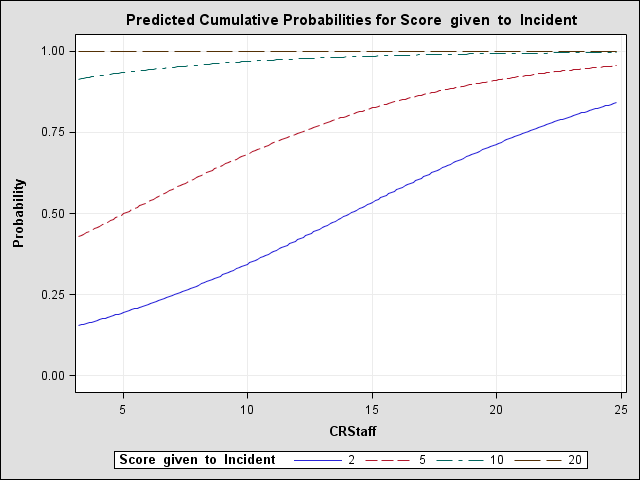
\includegraphics[scale=0.5]{Pic/Q6/1.png}
\caption{Predicted Cumulative Probabilities for Score Given to Incident}
\label{f12}
\end{figure}

The logistic model is used to fit the relationship between the severity of attack and the number of trained employees. According to the figure \ref{f12}, the more people are trained, the more obvious the probability of low-level injuries. This means that increasing the number of trainees will reduce the occurrence of high-level attacks, but not the number of attacks.
